%this section shall give a clear motivation (making tacit knowledge explicit)/some application examples (analysis (some example questions, see Berger et al. for motivation of these questions), communication, knowledge managament/transfer), include the FODA notation and show FeatureIDE examples (without analysis)
%=> how do we get from ad-hoc to our vision?

\subsection{Recap: Software Product Lines and Features}
\begin{frame}{\insertsubsection\ \mytitlesource{\fospl}}
	\leftorright{
		\mydefinition{Software Product Line}{
			\begin{itemize}
				\item set of software-intensive systems (aka products)
				\item sharing a common, managed set of features
				\item satisfying the needs of a domain
				\item developed from a common set of core assets (reuse)
			\end{itemize}
		}
		\href{https://commons.wikimedia.org/wiki/File:Geely_assembly_line_in_Beilun,_Ningbo.JPG}{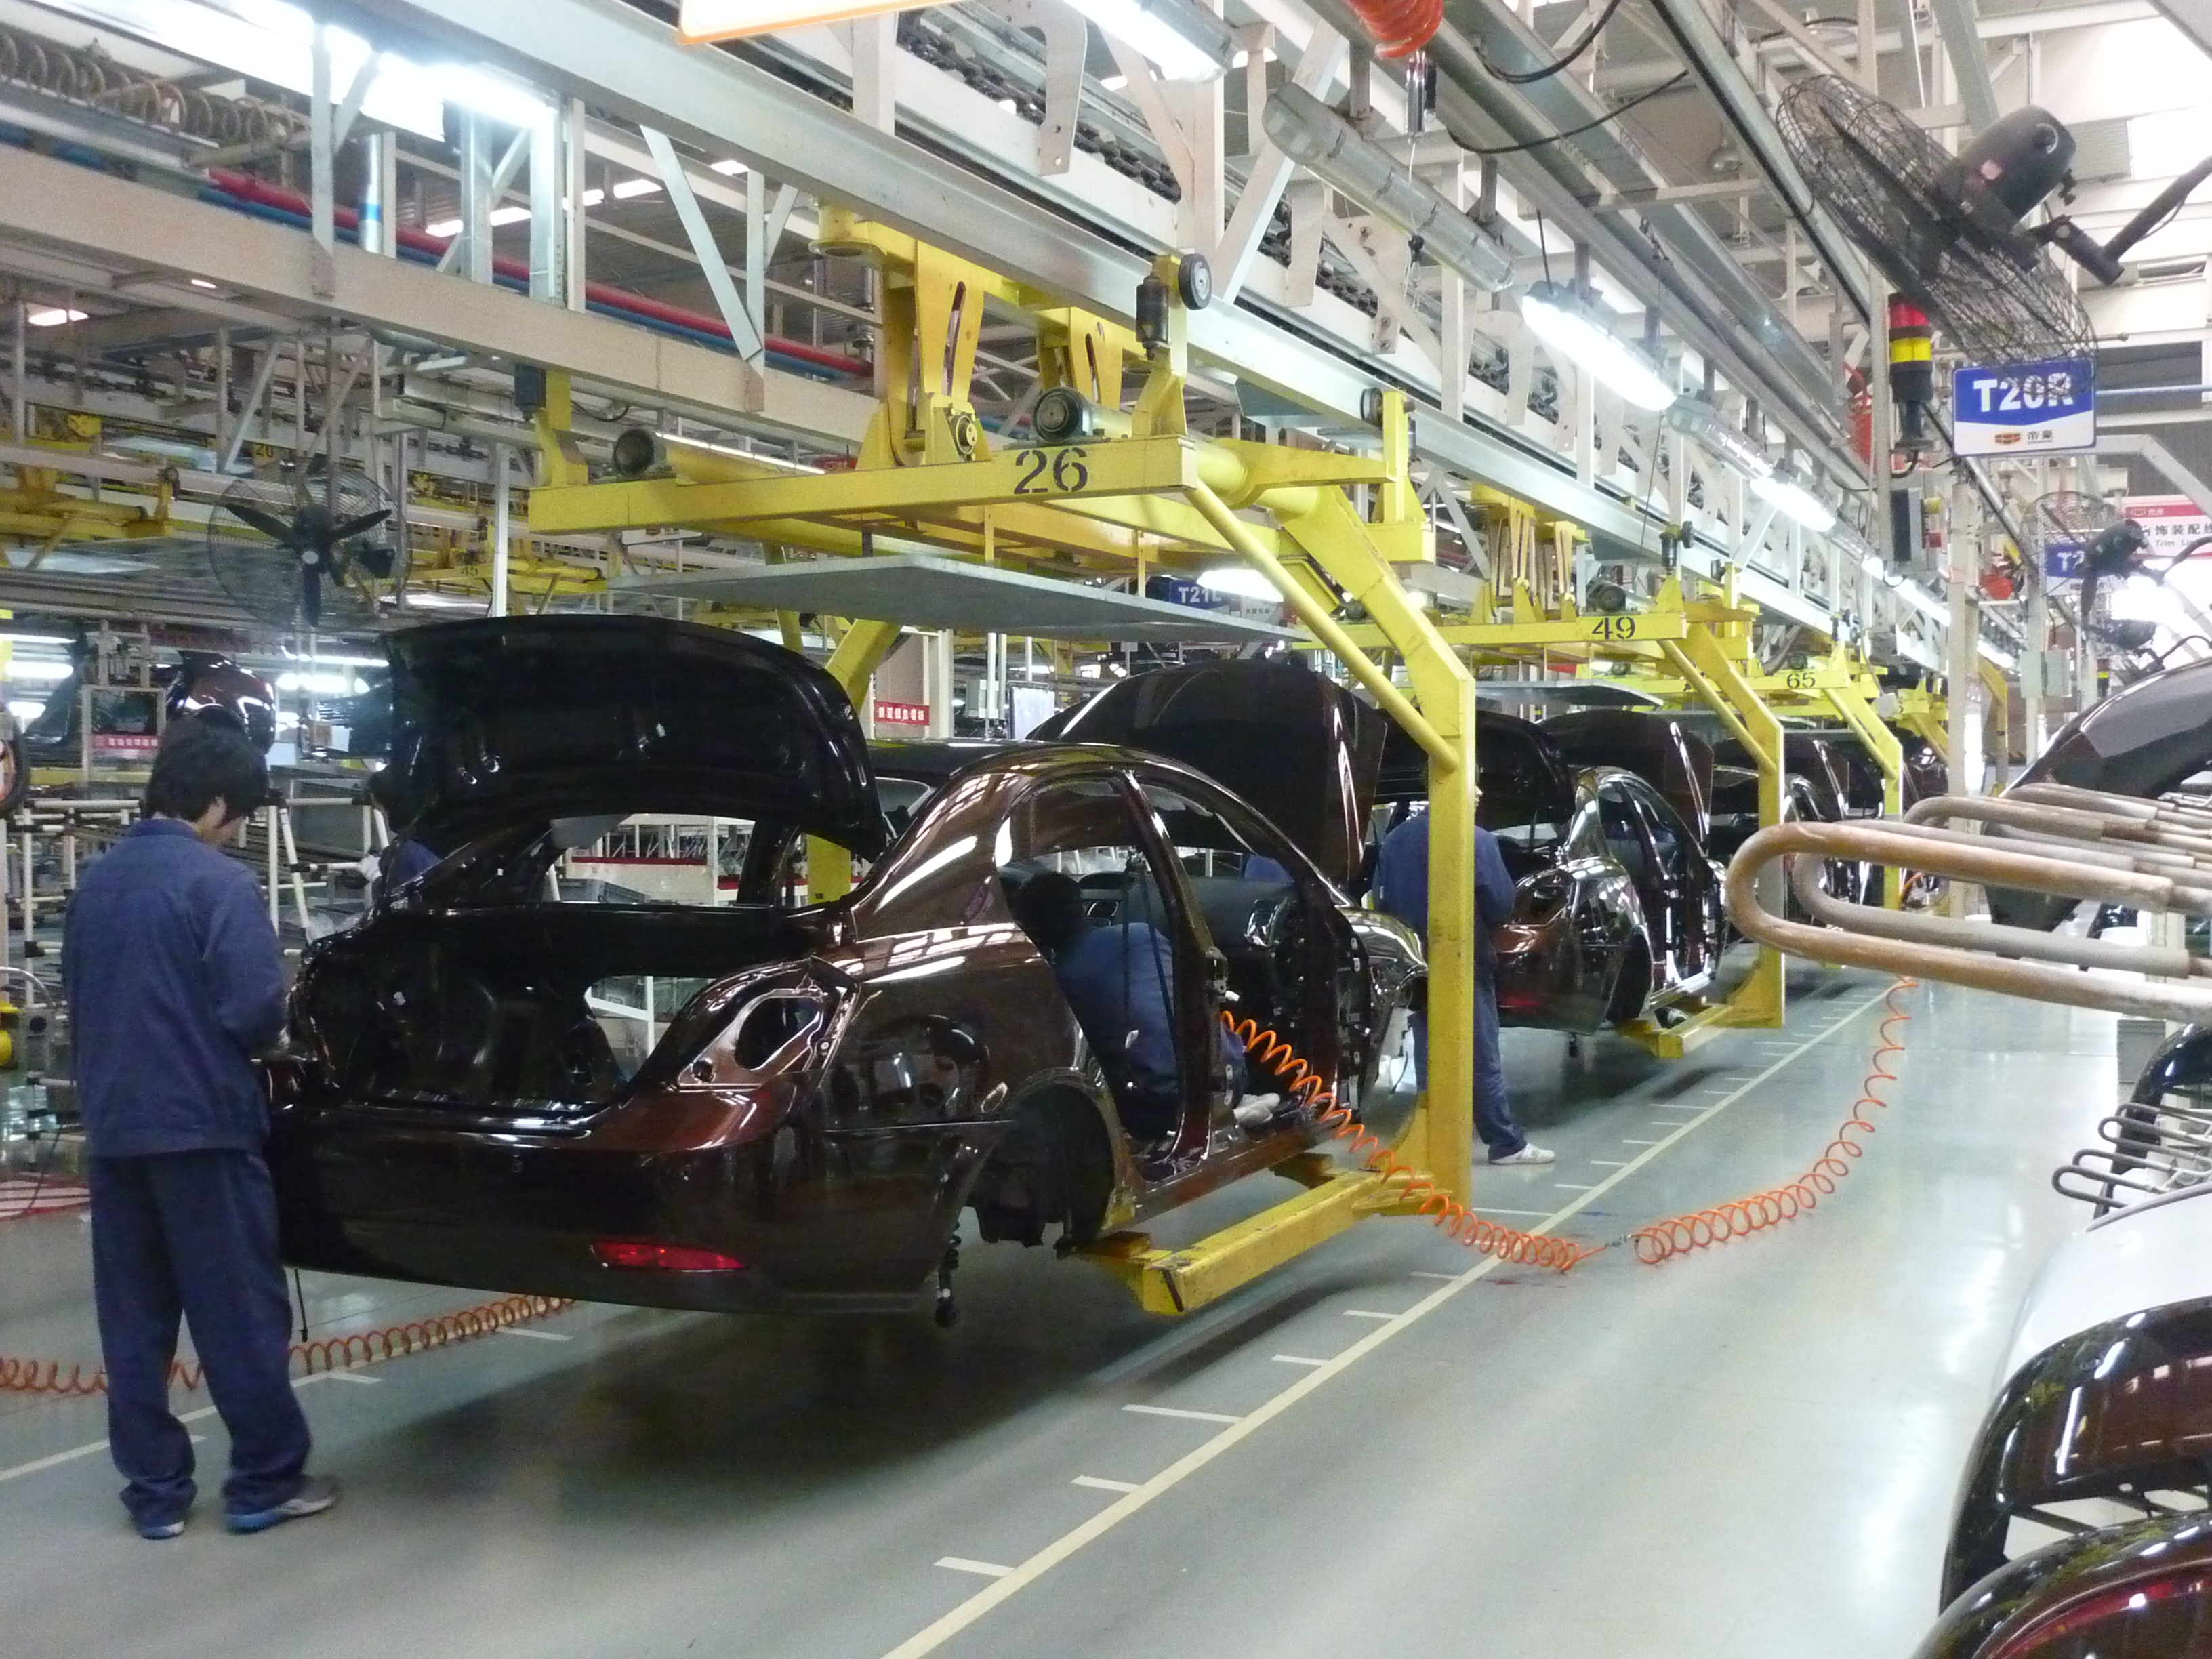
\includegraphics[width=\linewidth,trim=0 50 0 240,clip]{car-manufacturing}}
	}{
		\mydefinition{Feature}{
			\begin{itemize}
				\item domain abstraction
				\item used for communication by stakeholders (e.g., manager, developer, tester, customer, marketing)
				\item specifies differences between products
			\end{itemize}
		}
		\myexample{Examples}{
			\begin{itemize}
				\item \todots
			\end{itemize}
		}
		\todo{scoping?}
	}
\end{frame}

\subsection{Configuring Features}
\begin{frame}{\insertsubsection}
	\todo{examples for simple feature models without (or with few) dependencies}
	
	\todo{Configuring a Sandwich}

	\todo{Configuring ...}
\end{frame}

\xkcd{2369}

\subsection{Configuring Features with Dependencies}
\begin{frame}{\insertsubsection}
	\partofpage{70}{\myexampletight{Configuring a Notebook}{\only<1,3->{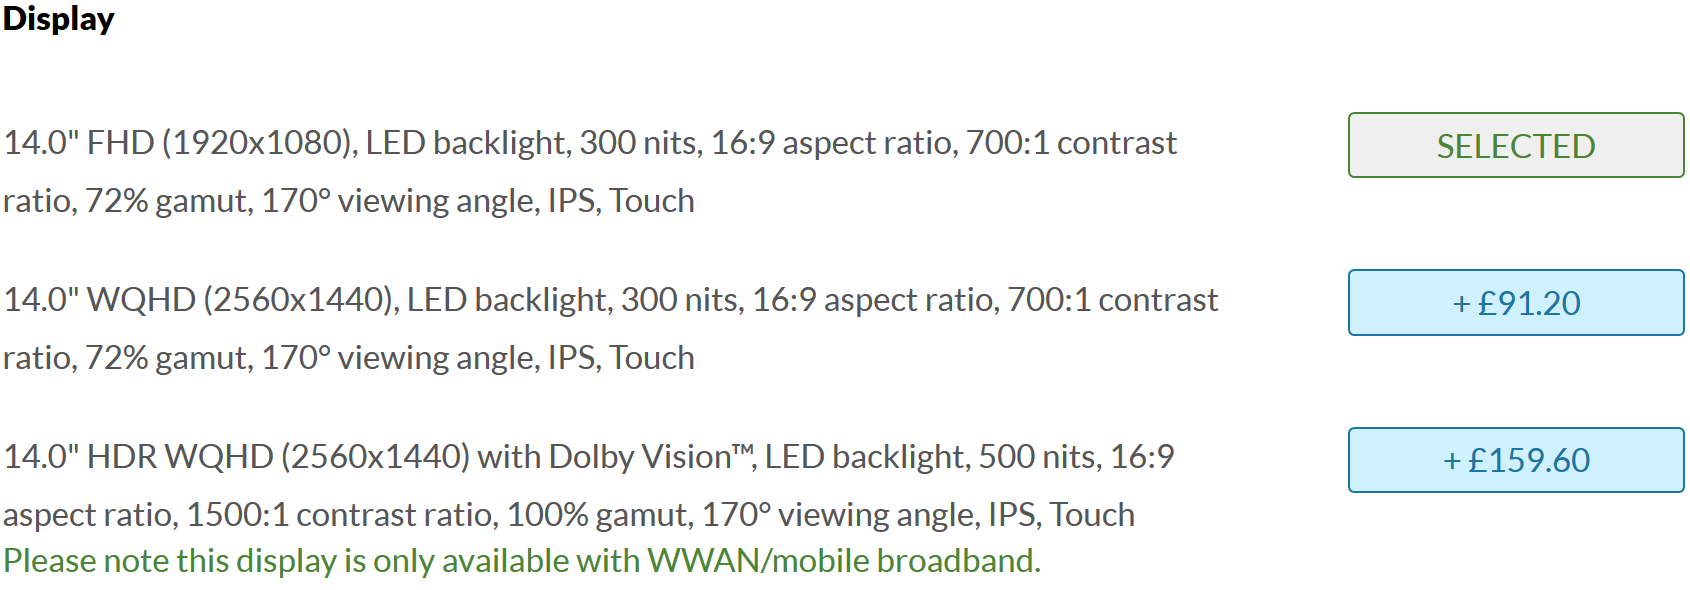
\includegraphics[width=\linewidth]{thinkpad-x1-yoga-display}}\only<2|handout:0>{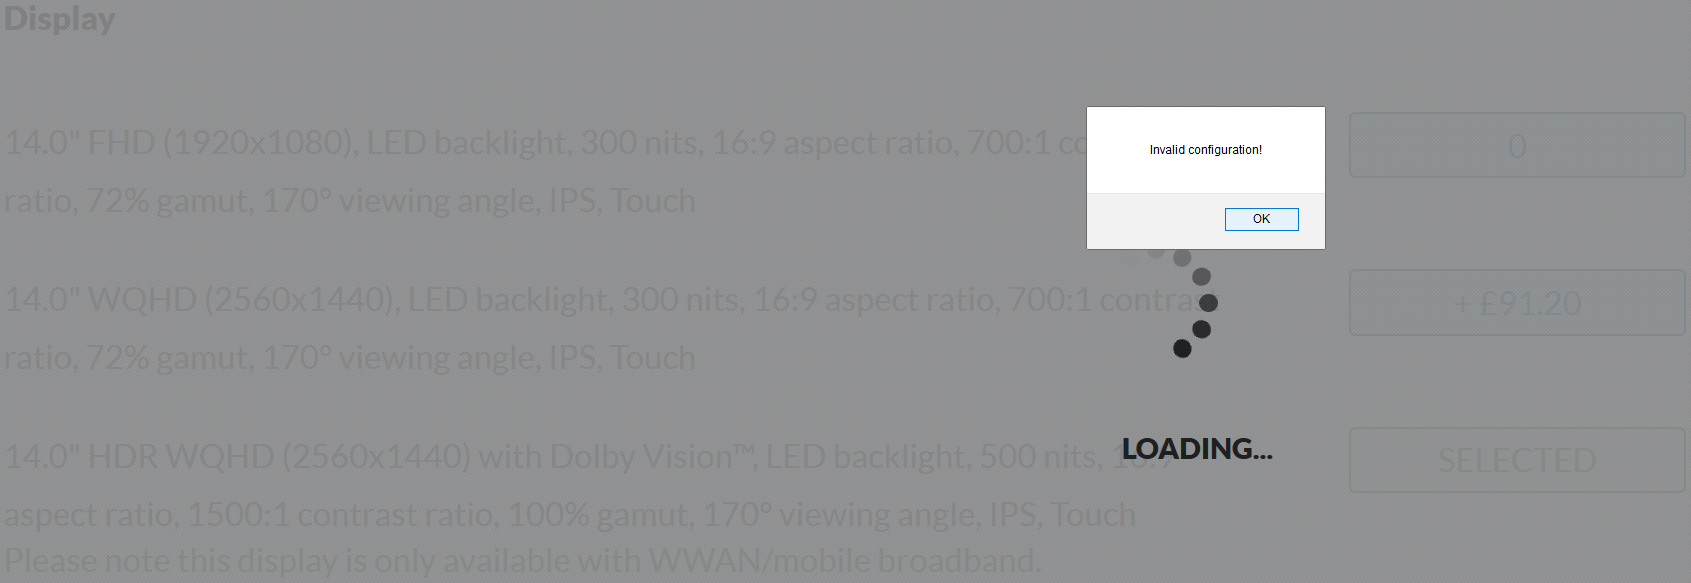
\includegraphics[width=\linewidth]{thinkpad-x1-yoga-display-invalidconf}}}}
\end{frame}

\begin{frame}{\insertsubsection}
	\partofpage{70}{\myexampletight{Still Configuring a Notebook}{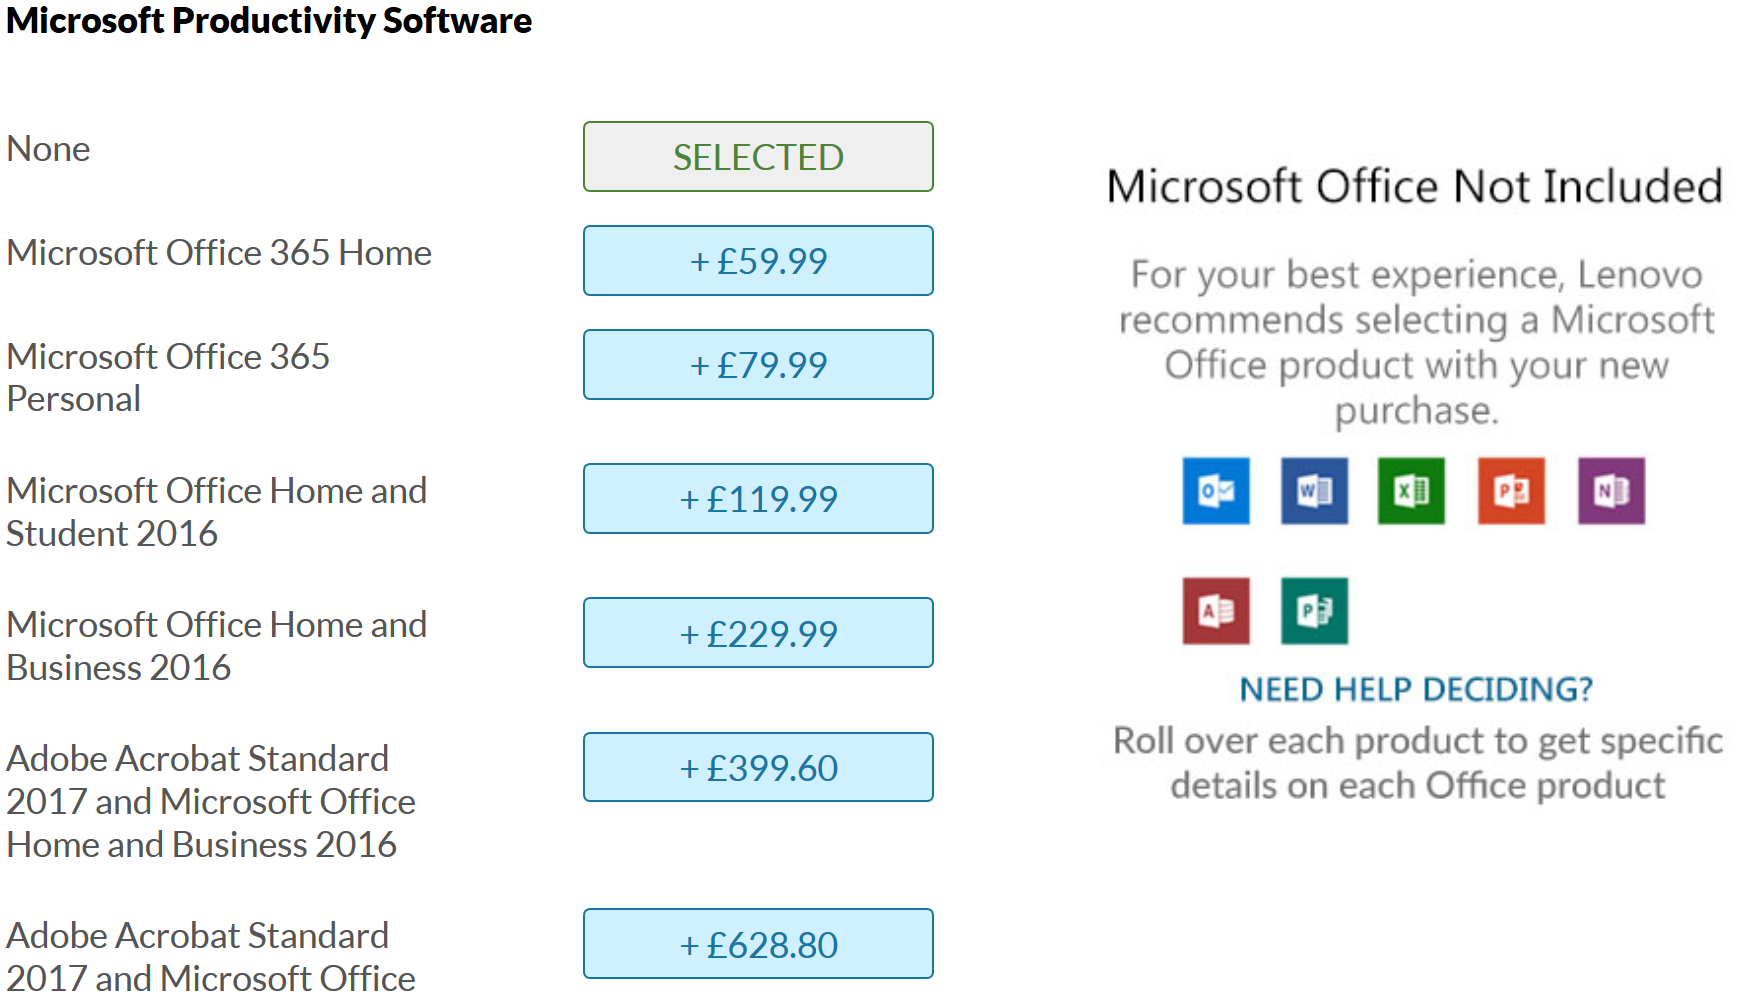
\includegraphics[width=\linewidth]{thinkpad-x1-yoga-office}}}
\end{frame}

\begin{frame}{\insertsubsection}
	~\hfill\partofpage{60}{\myexampletight{Configuring a Car}{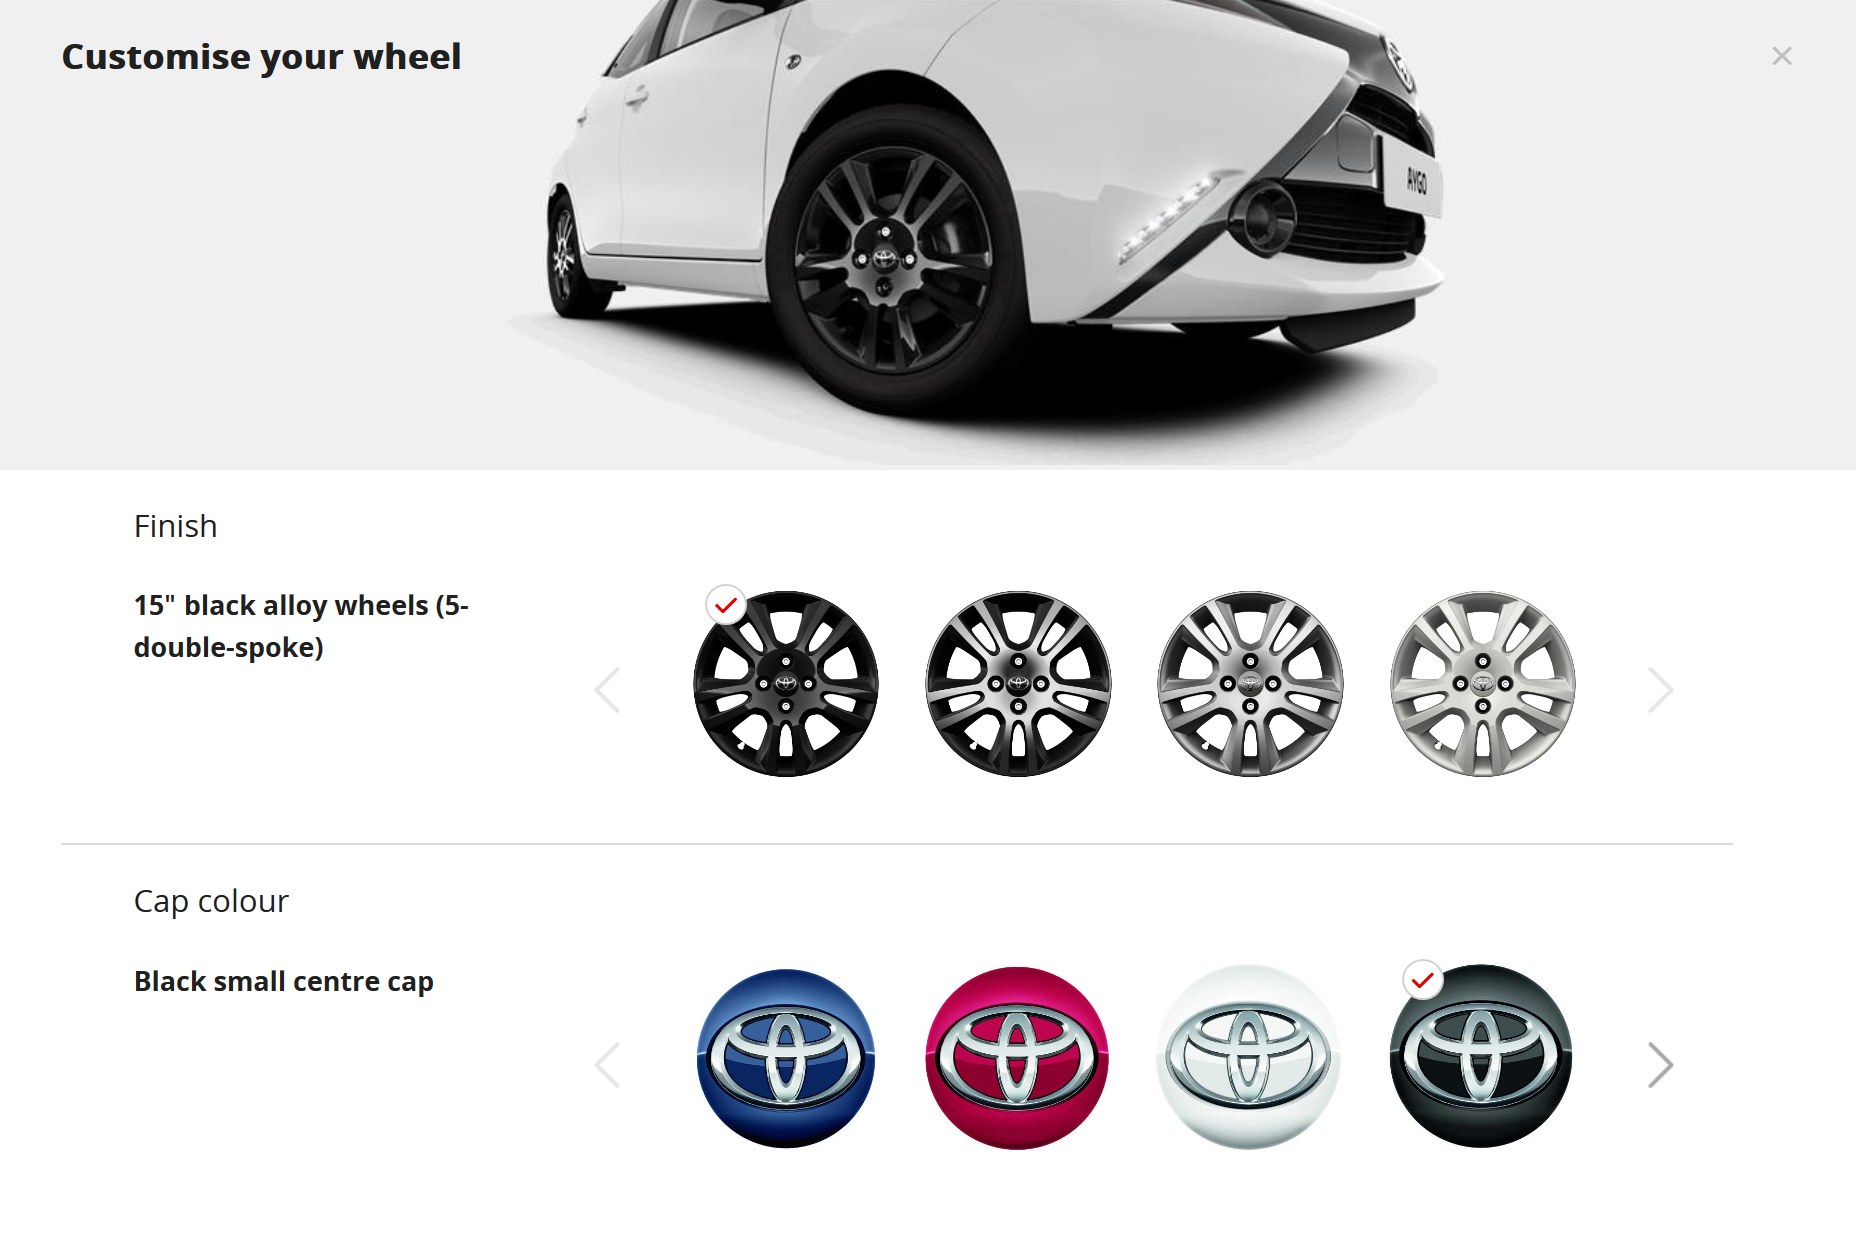
\includegraphics[width=\linewidth]{toyota-aygo-wheels}}}
\end{frame}

\begin{frame}{\insertsubsection}
	~\hfill\partofpage{60}{\myexampletight{Configuring a Car with a Weird Price}{\centering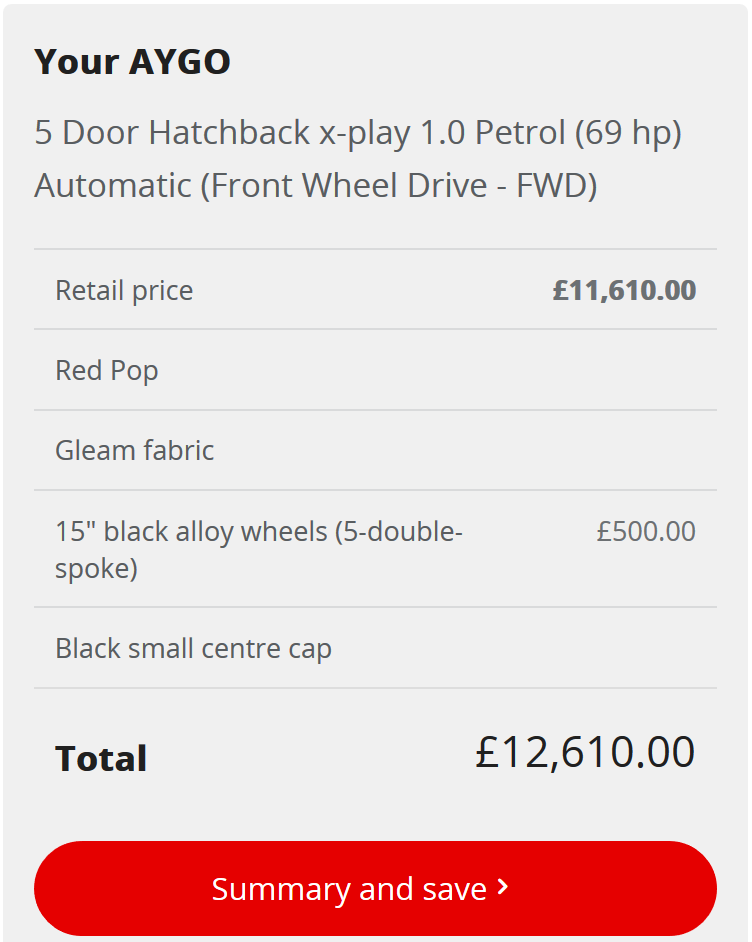
\includegraphics[width=.55\linewidth]{toyota-aygo-costs}}}
\end{frame}

\begin{frame}{\insertsubsection}
	~\hfill\partofpage{60}{\myexampletight{Configuring a Car with 8 Wheels!}{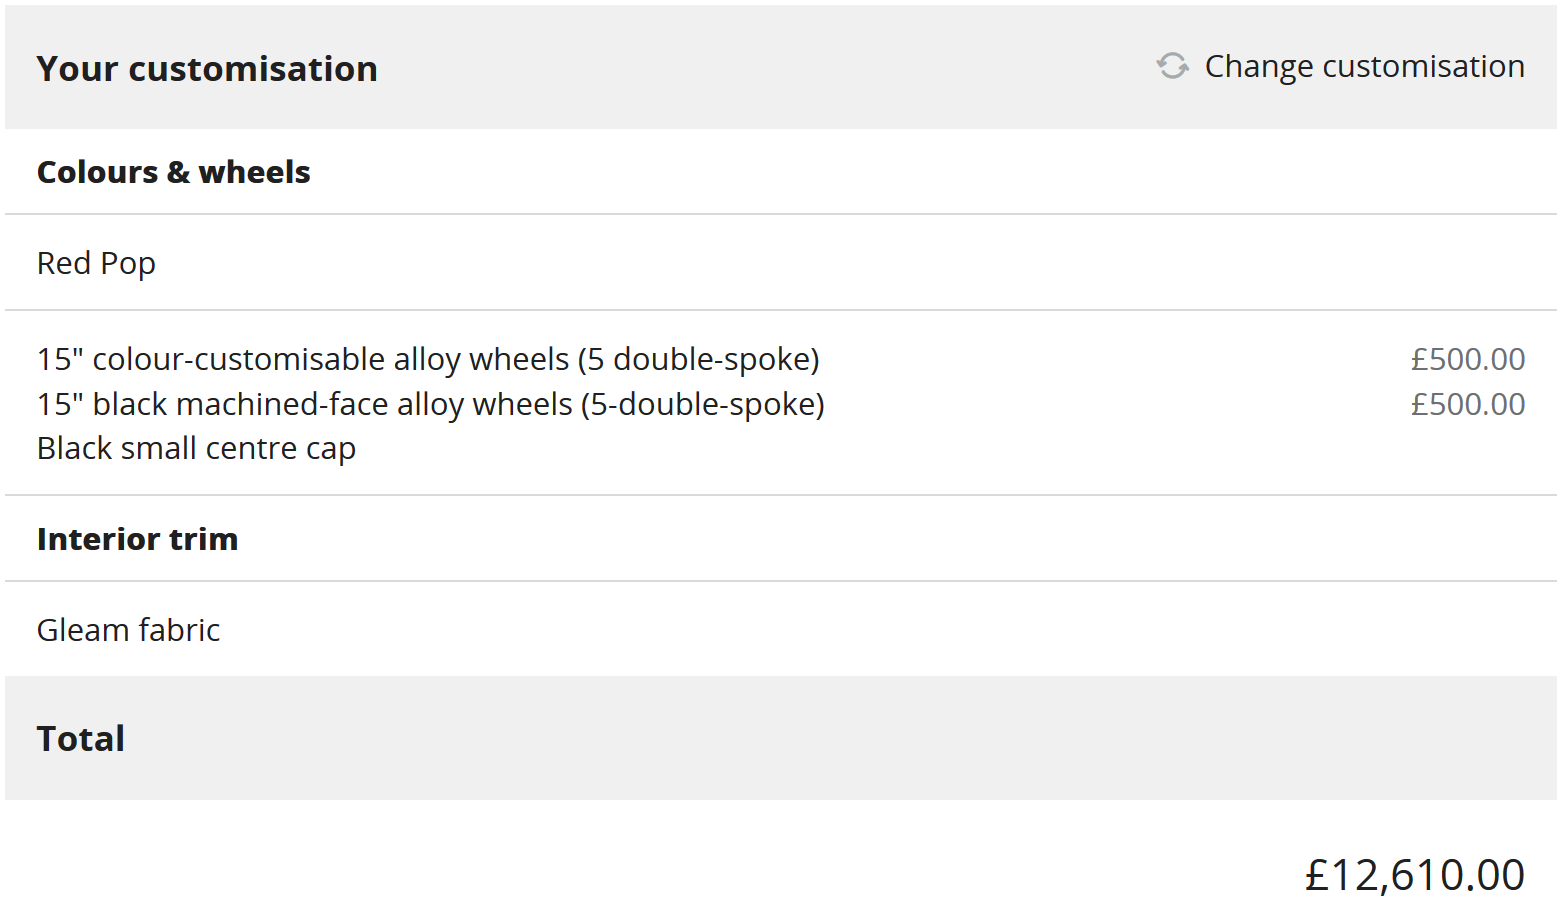
\includegraphics[width=\linewidth]{toyota-aygo-costs3}}}
\end{frame}

\begin{frame}{\insertsubsection}
	\partofpage{70}{\myexampletight{Configuring a German Car}{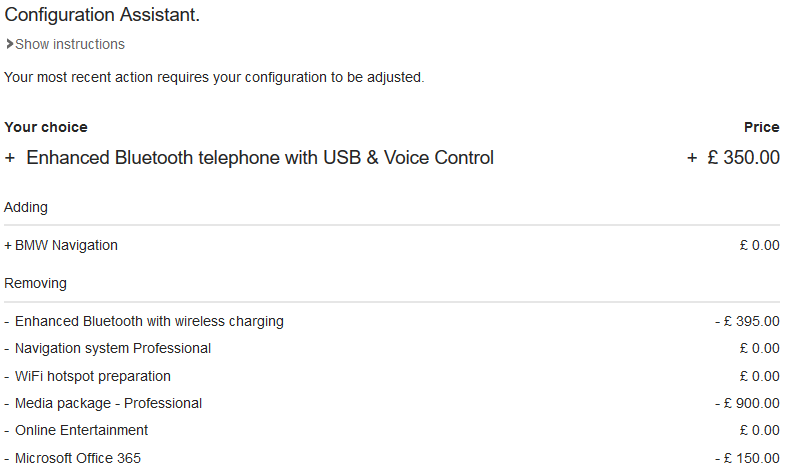
\includegraphics[width=\linewidth]{bmw-series1-confassistant-bluetooth}}}
\end{frame}

\subsection{Feature Diagrams}

\begin{frame}{\insertsubsection}
	a feature is( def?)
	a feature model is \ldots
	a cfg is....
\end{frame}

\newcommand{\dbmpl}{
	\myexampletight{A Database Management Product Line}{
		\centering
		\featureDiagramConfigurableDatabase\\
		$Transactions \pimplies Put \por Delete$

		\featureDiagramLegend
	}
}

\begin{frame}{\insertsubsection\ \mytitlesource{\fospl}}
	\leftorright{
		\dbmpl
	}{
		\mydefinition{Feature Diagram \todo{vs model?}}{ % graphical representation of feature models
			\begin{itemize}
				\item hierarchy of features
				\item dependencies between features modeled by tree and cross-tree constraints
				\item \emph{tree constraints}: defined by the hierarchy
				\item \emph{cross-tree constraints}: propositional formulas over features
				\item \emph{concrete features} have an implementation
				\item \emph{abstract features} are used to group other features
			\end{itemize}
		}
	}
\end{frame}

\begin{frame}{\insertsubsection\ \mytitlesource{\fospl}}
	\leftorright{
		\dbmpl
	}{
		\mydefinition{Tree Constraints}{
			\begin{itemize}
				\item each feature requires its parent
				\item an \emph{optional feature} \todo{has no further constraints}{can be (de-)selected freely when its parent is selected}
				\item a \emph{mandatory feature} is required by its parent
				\item \emph{or group}: at least one feature must be selected when the parent is selected
				\item \emph{alternative group}: exactly one feature must be selected when the parent is selected
			\end{itemize}
		}
		\mydefinition{Cross-Tree Constraints}{
			\begin{itemize}
				\item a list of propositional formulas expressing further dependencies between features
			\end{itemize}
		}
	}
\end{frame}

\begin{frame}{\insertsubsection\ \mytitlesource{\fospl}}
	\leftorright{
		\dbmpl
	}{
		% what is a cfg?
		\myexample{Valid Configurations}{ % one slide (gray out nonselected features)
			\begin{itemize}
				\item Read-only database on Windows:
					$\{CfgDB, Base, API, Get, OS, Win\}$
				\item Fully functional database on Unix:
					$\{CfgDB, Base, API, Get, Put, Delete, $\\
					$~Transactions, OS, Unix\}$
				\item \dots
			\end{itemize}
		}
		\myexample{Invalid Configurations}{ % one slide
			\begin{itemize}
				\item Violated tree constraint:
					$\{CfgDB, Base, API, OS\}$\\
					$\Rightarrow $ \emph{Get}, \emph{Put}, or \emph{Delete} missing; \emph{Windows} or \emph{Unix} missing
				\item Violated cross-tree constraint:
					$\{CfgDB, Base, API, Get, Trans., OS, Win\}$\\
					$\Rightarrow $ \emph{Put} or \emph{Delete} required by \emph{Transactions}
				\item \ldots
			\end{itemize}
		}
	}
\end{frame}

\begin{frame}{\insertsubsection\ \mytitlesource{\fospl}}
	\leftorright{
		\todo{other feature diagram example(s) which shows off how notation can also be used}
	}{
		\mynote{Notation}{
			\begin{itemize}
				\item abstract and concrete features can be assigned arbitrarily
    			\item groups can be used anywhere
				\item directly below groups, no optional or mandatory markers are allowed
			\end{itemize}
		}
	}
\end{frame}

\subsection{Advantages of Feature Modeling}
\begin{frame}{\insertsubsection}
	\leftandright{
		\textbf{Making Tacit Knowledge Explicit}
		\mynote{Interview with Practitioners \mysource{\href{https://link.springer.com/chapter/10.1007/978-3-319-11653-2_19}{Berger~et~al.~2014}}}{
			\mycite{I think the best [about feature modeling] is you can see relationships, to actually know what configurations are allowed and what are not allowed. That was also not so easy to express in the past [\ldots] This is from the developer’s point of view. But it’s also, we can see that from the, say project development, it’s also important, because before we noticed that \emph{the same functionality was implemented twice} within the same project, basically they haven’t realized that. They implemented the same features.}
		}
	}{
		\textbf{Tool Support for Automation}

		\todo{FeatureIDE, pure::variants screenshot?}
	}
\end{frame}

% advantages over Natural Language, List of Configurations